%The fwahl LaTeX template made for use at TU Eindhoven

\documentclass[11pt, a4paper, onecolumn, oneside, parskip=half]{scrartcl}

%%%%%%%SETUP BEGIN%%%%%%%
%Define constant names, etc.
\newcommand{\authors}{\\Stef Louwers (0590864)\\
Sunil Chokkanathapuram Ramanarayanan (0826874)\\
Qian Qian (0827493)\\
GROUP 3
} %List Authors here
\newcommand{\prof}{Prof. dr. Henk Corporaal, Lr. Roel S. Pieters, MSc, Lr. Mark Wijtvliet, MSc} %List Prof here
\newcommand{\doctitle}{Design and Implementation of a Quadcopter with Visual Control} %Document Title
\newcommand{\subcode}{5HC99} %Subject Code
\newcommand{\docsubject}{Embedded Visual Control} %Subject name, also appears in header
\newcommand{\centerhead}{S.T.Louwers, S.Chokkanathapuram Ramanarayanan, Q.Qian} %Center part of header
\newcommand{\centerfoot}{} %Center part of footer
%%%%%%%SETUP END%%%%%%%%
\usepackage{caption}
%\usepackage{subfigure}
\usepackage{subcaption}
\usepackage{graphicx}
\usepackage{amsmath}
\usepackage{listings}
\usepackage{a4wide}
\usepackage{color}
\usepackage{listings}
\usepackage{float}
\usepackage{amsmath}
\usepackage{booktabs}
\usepackage{footmisc}
\usepackage{sectsty}
\usepackage[headsepline,footsepline]{scrpage2}
\usepackage{hyperref}
\usepackage{titlesec}
\usepackage{placeins}
\usepackage{textcomp}

% Nonindented footnotes
\setlength{\footnotemargin}{2mm}

% Prevent PDF Version warnings
\pdfminorversion=6

% Colors
\definecolor{darkblue}{rgb}{0.0,0.0,1}
\definecolor{midgreen}{rgb}{0.0,0.5,0.0}
\definecolor{lightgray}{gray}{0.95}

% Listings
\lstset
{
	language=Verilog,
	frame=single,
	backgroundcolor=\color{lightgray},
	showstringspaces=false,
	keywordstyle=\bfseries\color{darkblue},
	commentstyle=\color{midgreen},
	basicstyle=\ttfamily\fontsize{8}{8}\selectfont,
	numbers=left,
	captionpos=b,
	breaklines=true,
	aboveskip=\baselineskip,
	tabsize=2
}

% New commands
\newcommand{\HRule}[2]{\noindent\rule[#1]{\linewidth}{#2}}
\newcommand{\vlinespace}[1]{\vspace*{#1\baselineskip}}
\newcommand{\todo}[1]{{\textcolor{red}{\textbf{TODO:} #1}}}

% TOC
\setcounter{tocdepth}{2}


% Header and footer
%\ihead{\docsubject{}}
\chead{\centerhead{}}
\ifoot{\headmark}
\cfoot{\centerfoot{}}
\ofoot{\thepage}
\automark[section]{section}

% Redefine headings
\titleformat{\section}{\sffamily\large\bfseries}{\thesection}{1em}{}
\titleformat{\subsection}{\sffamily\normalsize\bfseries}{\thesubsection}{1em}{}
\titleformat{\subsubsection}{\sffamily\normalsize\bfseries}{\thesubsubsection}{1em}{}
\titleformat{\paragraph}{\sffamily\normalsize\bfseries}{\theparagraph}{1em}{}
\titleformat{\subparagraph}{\sffamily\small\bfseries}{\thesubparagraph}{1em}{}

\begin{document}

\begin{titlepage}

\sffamily
\hfill \centering

\includegraphics[width=7cm]{tuelogo}
\HRule{11pt}{2pt}

\vfill
\Large{\docsubject{} \\\subcode{} \\}
\vlinespace{1}
\huge{\doctitle{}\\}
\vlinespace{8}
\vfill
\large
By \authors{}\\
\vfill
%\vlinespace{5}
\HRule{11pt}{2pt}
\raggedright
\textbf{Date: } \today \\
\textbf{Professor:} \prof{}

\end{titlepage}

\tableofcontents
\newpage
\pagestyle{scrheadings}

\section{Introduction}
In this project, a quadcopter is designed and implemented to autonomously fly and demonstrate on-board image processing capabilities. The project is aimed to control the quadcopter by virtue of two control systems; the local control, and the global control. The local control is intended for the stabilisation of the quadcopter, so that it is able to fly manually through the RC receiver and the global control is intended to make the quadcopter to fly autonomously with the aid of visual control through the camera. These two control loops are implemented on dedicated processors with appropriate capabilities.

% \section{Requirements}
% \section{Hardware}

\section{System Architecture}
In this section, we will discuss the used hardware and system architecture. First we will take a look at the local control, global control and used sensors, and after that, we will address communication used between these components.

\subsection{Local Control}
The local control is powered by an STM32F3Discovery development board, powered by the STM32F303VCT6 processor (a 72 MHz Cortex-M4 MCU), 48 KB RAM and 256 KB flash memory. This board also contains a gyroscope, accelerometer and a magnetic sensor, all measuring three axis. This makes it an ideal board for a quadcopter's local control, because it contains enough processing power, and has all the basic sensors available.

\subsection{Global Control}
For the global control, we have chosen for the Raspberry PI. We chose for this platform because it was cheap, we already had it available, and the camera module was expected soon after the start of the project.

Because we wanted two cameras on the quadcopter (one facing to the front, and one facing down), we decided to add two Raspberry PIs to the quadcopter, as each Raspberry PI only has the possibility to connect one camera. This also gave us more processing power available, as each Raspberry PI only has to process one camera.

\subsection{Sensors}
The local control board already contained the basic sensors required to fly a quadcopter: a gyroscope, an accelerometer and a magnetic sensor. To this list, we added a battery monitor, a barometer and two cameras.

\subsubsection{Battery monitor}
The battery monitor was a simple voltage divider that connected the battery voltage to one of the ADC pins of the STM32F3Discovery board. The voltage divider was necessary to convert the voltage to the 0 -- 3V domain.

\subsubsection{Barometer}
In order to facilitate altitude hold, we needed some means of measuring the current altitude of the quadcopter. Because other teams have reported some problems with the ultrasound sensor, we decided to do something different and try a barometer.

Compared to an ultrasound sensor, a barometer has less accuracy. Also, a barometer provides only a absolute height (to sea level). Thus a command like ``stay at 1 meter from the ground'' is not possible. Instead, we should say ``stay at the current height''. The advantage of the barometer over the ultrasound sensor is that it has no height limits, and that there are no false measurements as reported with the other groups.

\subsubsection{Cameras}
We have chosen for the Raspberry PI cameras, because they are affordable, of relative good quality, small and light, and they uses few system resources on the Raspberry PI. Because each Raspberry PI can only interface with one camera, we have placed two Raspberry PIs and cameras on the quadcopter.

These cameras are able to film in 1080p resolution with 30 fps, and take still images with 2592 x 1944 resolution.

\subsection{Communication}
There are many communication-paths, as can be seen in figure \ref{fig:communication}. In this section, these will all be discussed.

\begin{figure}[ht]
\centering
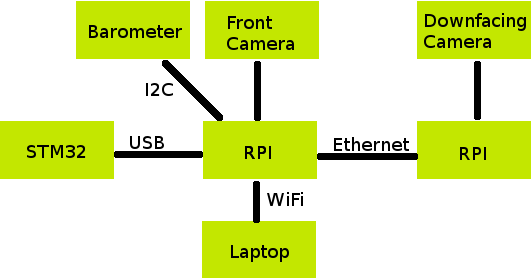
\includegraphics[width=0.6\textwidth]{hwdesign2}
\caption{Overview of different communication protocols.}
\label{fig:communication}
\end{figure}

\subsubsection{Local control and global control}
\label{sec:arch:comm:localglobal}
The local control on the STM32F3Discovery communicates with the first Raspberry PI using an USB-cable. They use the UAVTalk\footnote{\url{http://wiki.openpilot.org/display/Doc/UAVTalk}} protocol, and thus communicate high level objects. Because the UAVTalk protocol is already seamless integrated in the local control (it is also used for communication with the Ground Control Station), all useful pieces of data are available as a UAVObject.

This makes it an extremely powerful interface. Global control algorithms have access to all the information that it available to the local control, and it can influence and override all aspects of the local control by writing new values to these objects.

The interface is also flexible. Currently it uses USB, but UART or other protocols are also possible. The UAVObjects on the local control are also accessible on a laptop and on the other Raspberry PI, using a WiFi or an ethernet connection, thus eliminating the need for a separated (bluetooth) telemetry module.

A presentation on this topic is also available online on \url{http://youtu.be/uEVFPBQtt0U}.

\subsubsection{Raspberry PIs}
The two Raspberry PIs on the quadcopter need to be able to communicate, and they do this by a standard ethernet (network) cable. We chose for this option because it is supported out of the box and widely supported, and it is fast. Secondly, it allows the first Raspberry PI to share its WiFi connection easily with the second Raspberry PI, allowing easier remote management.

\subsubsection{Laptop}
On the Raspberry PI runs a normal Linux installation, and that gives the option to add a WiFi adaptor so that it can communicate with the outside world using WiFi. We did this, and even shared the internet connection to the second Raspberry PI, so both could easily download and install new software.

\subsubsection{Barometer}
The barometer is connected to the first Raspberry PI using I\texttwosuperior C. It is not connected to the STM32F3Discovery, because there where some problems with the I\texttwosuperior C driver in the TauLabs system, that we where unable to properly debug. The Raspberry PI sends the altitude information from the barometer to the STM32F3Discovery using the UAVObjects and the UAVTalk protocol, as discussed in section \ref{sec:arch:comm:localglobal}.

\subsubsection{Camera}
The cameras are attached to the Raspberry PIs, and use a flatcable for the connection to a CSI\footnote{Camera Serial Interface}-interface.

\section{Software}
\subsection{Local control}

\subsection{Global control}


\section{Objectives}

\subsection{Building Quadcopter and flying}

\subsection{Tuning Local control}

\subsection{Autonomous flight}

\subsection{360 degrees rotation}

\subsection{Altitude hold}

\subsection{Drift correction in horizontal axis}

\subsection{Camera capture while rotation}

\subsection{Stiching for Panorama image}

\subsection{On-board Marker identification on Global control}

\subsection{On-board Face detection}

\appendix
\newpage
\section{Who did what?}
% \begin{table}[ht!]
\begin{tabular}{ll}
Building the basic quadcopter & Stef, Sunil, Qian \\
Basic PID tuning & Stef, Sunil, Qian \\
More PID tuning & Stef \\
Attaching the cameras & Stef, Sunil \\
Battery monitor & Stef \\
Barometer & Stef \\
Writing the report & Stef \\
UAVTalk on Raspberry PI & Stef \\
Global control & Stef \\
\end{tabular}
% \end{table}
% \FloatBarrier

\section{Partlist}
\end{document}
